\documentclass[12pt, a4paper]{article}

\usepackage[utf8]{inputenc}

% Limit the page margin to only 1 inch.
\usepackage[margin=1in]{geometry}

%Imports biblatex package
\usepackage[
backend=biber,
style=alphabetic
]{biblatex}
%\addbibresource{../../mth342.bib}

% Enables the `align' environment.
\usepackage{amsmath}

% Provides useful environments, such as:
% - \begin{proof} ...\end{proof}
\usepackage{amsthm}
\newtheorem{proposition}{Proposition}
\theoremstyle{definition}
\newtheorem*{definition}{Definition}
\newtheorem{theorem}{Theorem}
\newtheorem{corollary}{Corollary}

% Enables using \mathbb{}, for example \mathbb{N} for the set of natural numbers.
\usepackage{amssymb}

% Allows using letters in enumerate list environment. Use, for example:
%\begin{enumerate}[label=(\alph*)]
% ...
%\end{enumerate}
\usepackage[inline]{enumitem}

% Enable importing external graphic files and provides useful commands, like \graphicspath{}
\usepackage{graphicx}
% Images are located in a directory called "images" in the current directory.
\graphicspath{{./images/}}

% Make links look better by default.
% See: https://tex.stackexchange.com/questions/823/remove-ugly-borders-around-clickable-cross-references-and-hyperlinks
\usepackage[hidelinks]{hyperref}
\usepackage{xcolor}
\hypersetup{
	colorlinks,
	linkcolor={red!50!black},
	citecolor={blue!50!black},
	urlcolor={blue!80!black}
}

% Code Listings. Source:
% https://stackoverflow.com/questions/3175105/inserting-code-in-this-latex-document-with-indentation
\usepackage{listings}
\usepackage{color}
\usepackage[most]{tcolorbox}

\definecolor{dkgreen}{rgb}{0,0.6,0}
\definecolor{gray}{rgb}{0.5,0.5,0.5}
\definecolor{mauve}{rgb}{0.58,0,0.82}

\lstset{frame=tb,
	language=Java,
	aboveskip=3mm,
	belowskip=3mm,
	showstringspaces=false,
	columns=flexible,
	basicstyle={\small\ttfamily},
	numbers=none,
	numberstyle=\tiny\color{gray},
	keywordstyle=\color{blue},
	commentstyle=\color{dkgreen},
	stringstyle=\color{mauve},
	breaklines=true,
	breakatwhitespace=true,
	tabsize=3
}

\newcommand{\prob}{\text{P}}
%\newcommand{\complement}{\mathsf{c}}
\title{Lecture 7: MATH 342W: Introduction to Data Science and Machine Learning}
\author{Sergio E. Garcia Tapia\thanks{Based on lectures of Dr. Adam Kapelner at Queens College.
See also the \href{https://github.com/kapelner/QC_MATH_342W_Spring_2025}{course GitHub page}.}}
\date{February 20, 2025 (last updated \today)}

\begin{document}
	\maketitle
	\section*{Estimating Covariance}
	Last time, we introduced ordinary least squares regression for $p=1$ and derived the following
	expressions for the least squares estimates:
	\begin{align}
		b_0 &= \bar{y} - b_1 \bar{x}\label{eqn:ols_b0}\\
		b_1 &= r\frac{S_y}{S_x}\label{eqn:ols_b1_r}\\
		r &= \frac{S_{xy}}{S_xS_y}\nonumber
	\end{align}
	where
	\begin{align}
		S_x^2  &:= \frac{1}{n-1}\sum_{i=1}^{n}(x_i-\bar{x})^2\nonumber\\
		S_y^2  &:= \frac{1}{n-1}\sum_{i=1}^{n}(y_i-\bar{y})^2\nonumber\\
		S_{xy} &:= \frac{1}{n-1}\sum_{i=1}^{n}(x_i-\bar{x})(y_i-\bar{y})\label{eqn:cov_xy_estimate}
	\end{align}
	The quantities $S_x^2$ and $S_y^2$ estimate the variance of $\sigma_x^2$ and $\sigma_y^2$,
	respectively (the variances of $x$ and $y$). This is similar to how $\bar{x}$ seeks
	to estimate $\mu_X$ and $\bar{y}$ seeks to estimate $\mu_Y$. The quantity $S_{xy}$
	estimates the \emph{covariance} of $x$ and $y$, given by
	\begin{align*}
		Cov[X, Y] := E[(X-\mu_X)(Y-\mu_Y)]
	\end{align*}
	where $X$ and $Y$ are random variables, $\mu_X$ and $\mu_Y$ are their respective means,
	and $E$ is used to compute the expectation. Though not a core part of this course, we
	will briefly talk about the meaning of $Cov[X, Y]$, and we'll use the estimate
	in $S_{xy}$ from Equation~\ref{eqn:cov_xy_estimate}.
	\subsubsection*{Case 1: $S_{xy} > 0$}
	Consider the data set depicted in Figure~\ref{fig:dataset-positive_{sxy}}.
	\begin{figure}
		\centering
		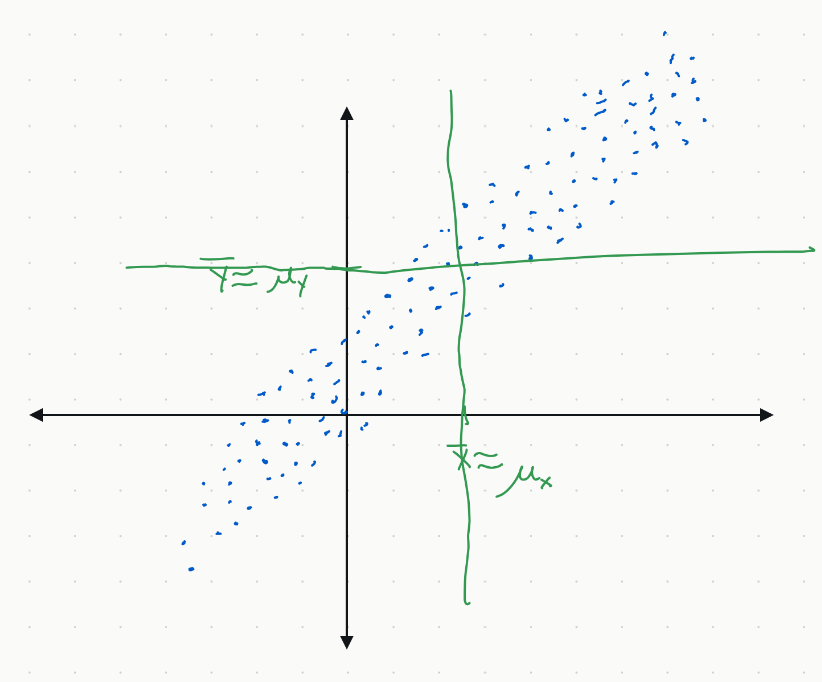
\includegraphics[width=0.5\textwidth]{positive-covariance-rvs}
		\caption{A data set where $S_{xy}>0$}
		\label{fig:dataset-positive_{sxy}}
	\end{figure}
	We've plotted a vertical and horizontal line through $\bar{x}$ and $\bar{y}$. This causes
	the plane to be partitioned into four regions. We focus on two cases:
	\begin{enumerate}[label=(\roman*)]
		\item If $x_i\geq \bar{x}$, we see that $y_i$ tends to be above the mean.
		Now $(x_i - \bar{x})\geq 0$, and $(y_i-\bar{y})$ is mostly positive also.
		Therefore, the product is mostly positive.
		\item If $x_i < \bar{x}$, we see that $y_i$ tends to be below the mean.
		Now $(x_i-\bar{x})<0$, and $(y_i-\bar{y})$ is mostly negative also.
		Once again, the product tends to be positive.
	\end{enumerate}
	Thus, in this case we have $S_{xy}>0$.
	\subsubsection*{Case 2: $S_{xy} < 0$}
	In Figure~\ref{fig:dataset-negative_{sxy}}, we've plotted a different data set.
	\begin{figure}
		\centering
		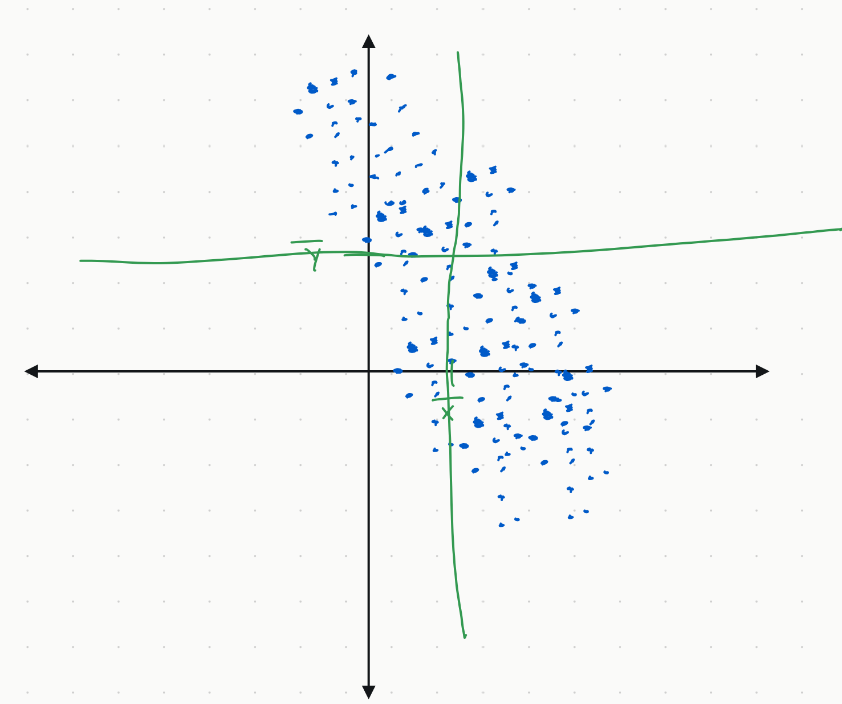
\includegraphics[width=0.5\textwidth]{negative-covariance-rvs}
		\caption{A data set where $S_{xy}<0$}
		\label{fig:dataset-negative_{sxy}}
	\end{figure}
	Once again, we've plotted
	the vertical and horizontal lines through $\bar{x}$ and $\bar{y}$, respectively. This causes
	the plane to be partitioned into four regions like before. We focus on two similar
	cases:
	\begin{enumerate}[label=(\roman*)]
		\item If $x_i\geq \bar{x}$, we see that $y_i$ tends to be below the mean.
		Now $(x_i - \bar{x})\geq 0$, and $(y_i-\bar{y})$ is mostly negative also.
		Therefore, the product is mostly negative.
		\item If $x_i < \bar{x}$, we see that $y_i$ tends to be above the mean.
		Now $(x_i-\bar{x})<0$, and $(y_i-\bar{y})$ is mostly positive also.
		Once again, the product tends to be negative.
	\end{enumerate}
	Thus, in this case we have $S_{xy}<0$.
	\subsubsection*{Case 3: $S_{xy} = 0$}
	For this last case, we've plotted points in Figure~\ref{fig:dataset-zero_{sxy}} such
	that they appear to be distributed like a disk roughly around the point $(\bar{x}, \bar{y})$.
	\begin{figure}
		\centering
		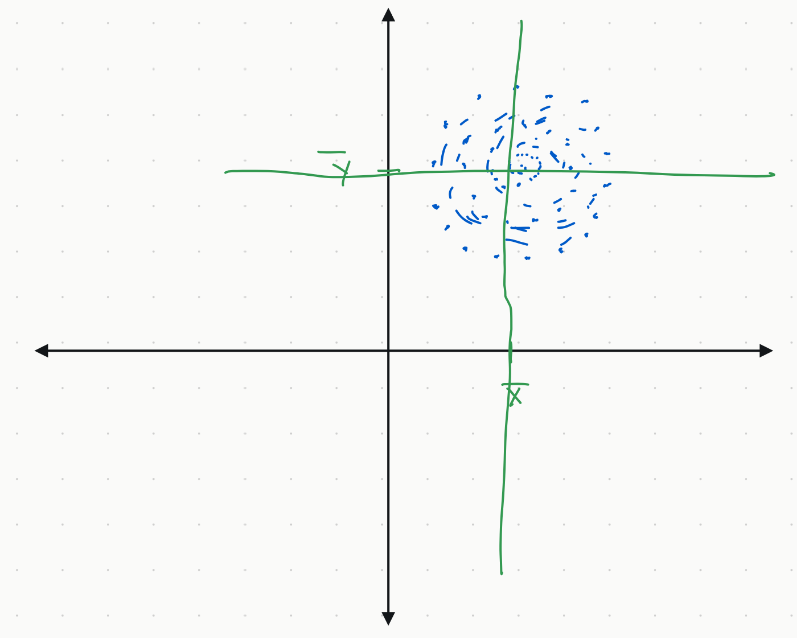
\includegraphics[width=0.5\textwidth]{zero-covariance-rvs}
		\caption{A data set where $S_{xy}\approx0$}
		\label{fig:dataset-zero_{sxy}}
	\end{figure}
	\begin{enumerate}[label=(\roman*)]
		\item If $x_i\geq \bar{x}$, we see that $y_i$ tends to be above the mean just
		as often as it is below the mean, so on average, we see $(y_i-\bar{y})\approx 0$.
		Therefore, the product is mostly positive.
		\item If $x_i < \bar{x}$, we see the same behavior.
	\end{enumerate}
	Therefore, in this case we have $S_{xy}\approx 0$.
	\subsubsection*{Interpretation}
	Having observed the previous three cases and considered the estimates $S_{xy}$,
	what can we say about $Cov[X, Y]$? It measures the degree and direction of the
	linear relationship between $X$ and $Y$ in units of $x$ times $y$. For example,
	if $x$ is measured in kilograms (kg) and $y$ is measured in meters (m), then
	the units of $S_{xy}$ are kilograms-meters (kg-m).
	Meanwhile, the quantity $r=S_{xy}/S_xS_y$ is unitless.
	\section*{Least Squares Facts}
	\begin{tcolorbox}[breakable=true]
		\begin{theorem}
			\label{thm:zero-sum-residuals}
			Suppose $\mathbb{D}=\{(x_i,y_i)\}_{i=1}^{n}$ is a data set where each $x_i,y_i\in\mathbb{R}$.
			If $b_0$ and $b_1$ are the ordinary least square estimates, $\hat{y}_i$ is the prediction
			corresponding to $x_i$ using the least squares estimates, and $e_i=y_i-\hat{y}_i$ is the
			residual for the $i$th response, then the sum of the residuals is zero:
			\begin{align*}
				\sum_{i=1}^{n}e_i=0
			\end{align*}
		\end{theorem}
		\begin{proof}
			Given the least squares estimates in Equations~\ref{eqn:ols_b0}~and~\ref{eqn:ols_b1_r},
			the linear model is $g(x)=b_0+b_1x$. In particular, $\hat{y}_i=g(x_i)+b_0+b_1 x_i$,
			so
			\begin{align*}
				\sum_{i=1}^{n}e_i &= \sum_{i=1}^{n}(y_i-\hat{y}_i)\\
				&=\sum_{i=1}^{n}(y_i-g(x_i))\\
				&=\sum_{i=1}^{n}(y_i-b_0-b_1x_i)\\
				&=\sum_{i=1}^{n}y_i-b_0\sum_{i=1}^{n}(1)-b_1\sum_{i=1}^{n}x_i\\
				&=n\bar{y}-nb_0-b_1n\bar{x}\\
				&=n(\underbrace{\bar{y}-b_1\bar{x}}_{b_0}-b_0)\\
				&=n(b_0-b_0)\\
				&=0.
			\end{align*}
		\end{proof}
	\end{tcolorbox}
	\begin{tcolorbox}[breakable]
		\begin{corollary}
			\label{coroally:zero-mean-residuals}
			The mean of the residuals in OLS is zero: $\overline{e}=0$.
		\end{corollary}
	\end{tcolorbox}
	\begin{tcolorbox}[breakable]
		\begin{theorem}
			Let $\mathbb{D}=\{(x_i,y_i)\}_{i=1}^{n}$ be a data set with $x_i,y_i\in\mathbb{R}$,
			and let $b_0,b_1$ be the least squares estimates. If $\overline{x}$ and $\overline{y}$
			denote the averages of the $x_i$'s and $y_i$'s respectively, then the point
			$(\overline{x}, \overline{y})$ lies on the least squares line defined by the
			estimates.
		\end{theorem}
		\begin{proof}
			Since $g(x)=b_0 + b_1x$, we can once again use Equation~\ref{eqn:ols_b0} to conclude that
			\begin{align*}
				g(\overline{x}) = b_0 + b_1\overline{x} = (\overline{y} - b_1\overline{x}) + b_1\overline{x}
				= \overline{y}.
			\end{align*}
		\end{proof}
	\end{tcolorbox}
	\section*{The Performance of the Linear Least Squares Model}
	Recall that OLS was introduced when moving to a numeric response space,
	i.e., $\mathcal{Y}=\mathbb{R}$. We began by considering the simple case
	where $p = 1$. In this setting, we saw that the null model $g_0=\bar{y}$.
	That is, the null model always predicts $\bar{y}$. This too is a linear
	model, with a slope of $0$ and an intercept of $\overline{y}$.
	Figure~\ref{fig:ols-null-model} illustrates the null model when $p=1$.
	\begin{figure}
		\centering
		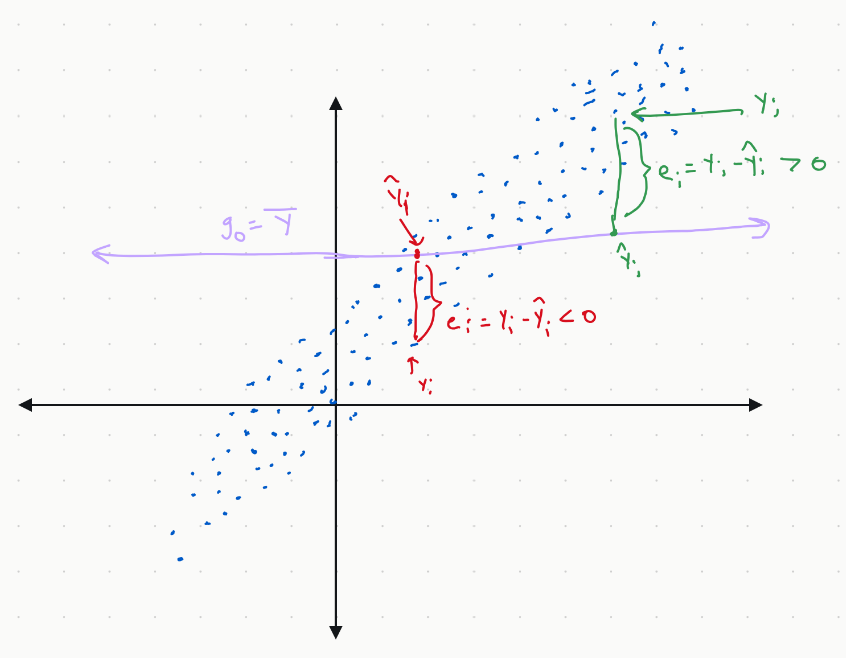
\includegraphics[width=0.8\textwidth]{ols-null-model}
		\caption{The null model in OLS with $p=1$.}
		\label{fig:ols-null-model}
	\end{figure}
	Notice how the residuals $e_i=y_i-\bar{y}_i$ are positive for points above the graph of
	$g_0$ and negative for points below the graph of $g_0$. One way to think about
	the performance of the null model is to view the distribution of the residuals,
	as illustrated in Figure~\ref{fig:ols-null-model-residuals}.
	\begin{figure}
		\centering
		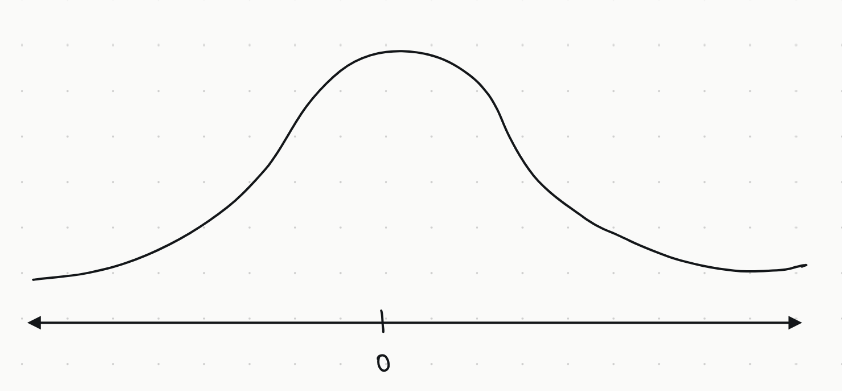
\includegraphics[width=0.6\textwidth]{ols-residuals-distribution-null-model}
		\caption{The distribution of the residuals in the null model in Figure~\ref{fig:ols-null-model}.}
		\label{fig:ols-null-model-residuals}
	\end{figure}
	Notice how this distribution is centered around $0$, which is consistent with the
	fact that $\bar{e} = 0$, as in Corollary~\ref{coroally:zero-mean-residuals}.
	
	We seek to compare the performance of the null model with the least squares
	estimates by comparing the distribution of the residuals. Figure~\ref{fig:ols-least-squares-model}
	shows the linear model defined by the least squares estimates (Equations~\ref{eqn:ols_b0}~and~
	\ref{eqn:ols_b1_r}).
	\begin{figure}
		\centering
		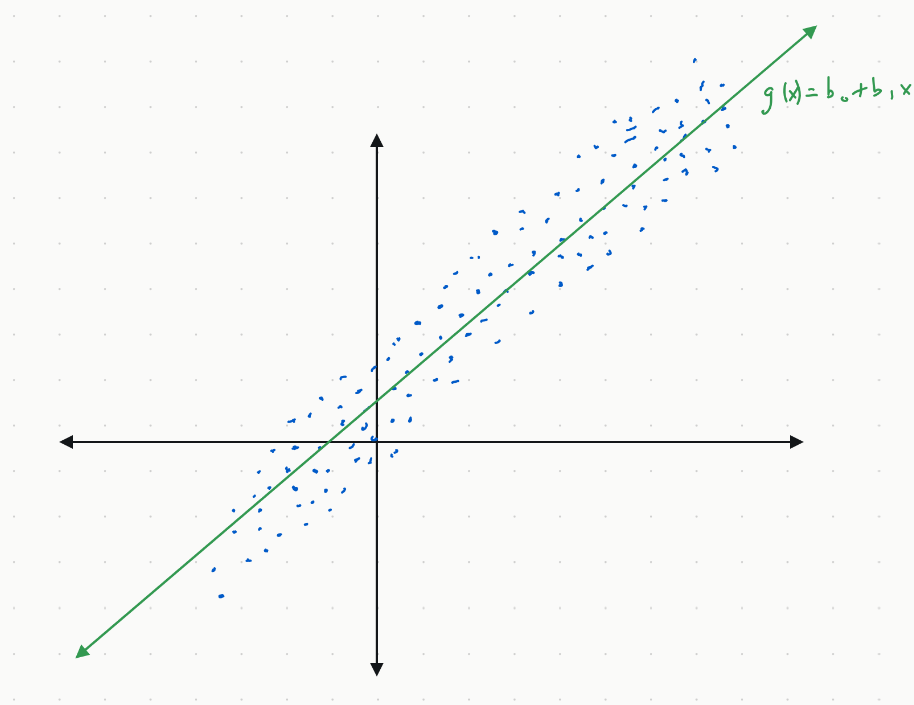
\includegraphics[width=0.6\textwidth]{ols-least-squares-estimate}
		\caption{The least squares model for the same data set as in Figure~\ref{fig:ols-null-model}.}
		\label{fig:ols-least-squares-model}
	\end{figure}
	In Figure~\ref{fig:ols-residuals-distribution-least-squares}, we see the
	corresponding distribution of the residuals.
	\begin{figure}
		\centering
		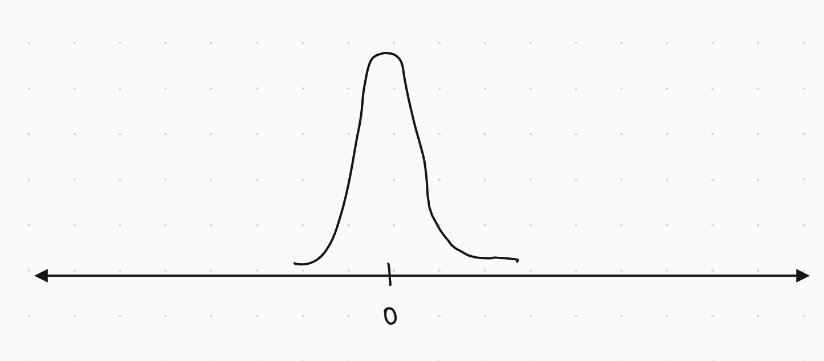
\includegraphics[width=0.6\textwidth]{ols-residual-distribution-least-squares-model}
		\caption{Distribution of the residuals in the model in Figure~\ref{fig:ols-least-squares-model}.}
		\label{fig:ols-residuals-distribution-least-squares}
	\end{figure}
	Notice that similar to $g_0$, the distribution of the residuals is centered at $0$,
	but it has a smaller variance compared to $g_0$. In fact, we will later show that this
	is always the case for OLS\footnote{Based on our discussion on covariance, we can also
		better understand the effect of $r$ in Equation~\ref{eqn:ols_b1_r}. The quantities
		$S_x$ and $S_y$ are estimations
		of the standard deviation of $x$ and $y$, respectively, so they are positive quantities.
		Meanwhile, as we saw, $r=S_{xy}/S_xS_y$, and its sign is dictated by $S_{xy}$.
		Hence, the slope of the least squares regression line is $b_1$, whose sign is determined
		by $r$, which in turn has its sign determined by $S_{xy}$.
	}.
	\subsection*{The Variance in the Residuals}
	Let $E_0$ be a random variable for the residuals of the null model $g_0$,
	and consider the variance $\sigma_0^2$ of $E_0$:
	\begin{align*}
		\sigma_{0}^2 := \text{Var}[E_0] := E[(E_0-\mu_{E_0}^2)]
	\end{align*}
	where $E[\cdot]$ stands for expectation, and $\mu_{E_0}$ stands for the mean
	of $E_0$. As we've seen, the variance is estimated by $S^2_{e_0}$
	(where now we use lowercase $e_0$ for the \emph{realization} of the
	random variable $E_0$). By Corollary~\ref{coroally:zero-mean-residuals}, we
	know $\overline{e}=0$. Recalling that the model always predicts $\overline{y}$,
	we can show that
	\begin{align*}
		S_{e_0}^2 &:= \frac{1}{n-2}\sum_{i=1}^{n}(e_i-\bar{e})^2\\
		&=\frac{1}{n-2}\sum_{i=1}^{n}e_i^2\\
		&=\frac{1}{n-2}\sum_{i=1}^{n}(y_i-\hat{y}_i)^2\\
		&=\frac{1}{n-2}\sum_{i=1}^{n}(y_i-\bar{y})^2
		\tag{$\hat{y}_i=\bar{y}$ for $g_0$}\\
		&:=\frac{1}{n-2}SSE_0,
	\end{align*}
	where we use the symbol $SSE_0$ to denote the sum of squared errors for the null model.
	The sum of squared errors for the null model is also called the \emph{sum of squared totals},
	or $SST$.
	\begin{tcolorbox}[breakable]
		\begin{definition}
			Given a finite sequence of values $(y_i)_{i=1}^{n}$ with average $\overline{y}$,
			the \textbf{sum of squared totals}, or SST, is defined by
			\begin{align*}
				SST := SSE_0 = \sum_{i=1}^{n}(y_i-\bar{y})
			\end{align*}
			The $SST$ is the $SSE$ of the null model $g_0$.
		\end{definition}
	\end{tcolorbox}
	Now let $E_g$ be the random variable for the residuals of the least square model $g$.
	Once again, we consider the variance in $E$
	\begin{align*}
		\sigma_{E_g}^2 := \text{Var}[E_g] := E[(E-\mu_{E_g}^2)]
	\end{align*}
	which is estimated by $S_{e_g}^2$ (noticed again lowercase $e_g$ for the realization of $E_g$)
	\begin{align*}
		S_{e_g}^2 &:= \frac{1}{n-2} \sum_{i=1}^{n}(e_{g,i}-\overline{e}_g)^2\\
		&=\frac{1}{n-2}\sum_{i=1}^{n}e_{g,i}^2
		\tag{$\bar{e}_g=0$ by Corollary~\ref{coroally:zero-mean-residuals}}\\
		&=\frac{1}{n-2}\sum_{i=1}^{n}SSE_g\\
		&:=MSE_g
	\end{align*}
	where $MSE_g$ is the mean-squared error of $g$ and $SSE_g$ is the sum of squared errors of $g$.
	The relations shown reveal why $SSE_g$ is an important performance metric: it is related
	to the variance in the errors of the residuals.
	\subsection*{The $R^2$ Performance Metric}
		
	In literature, $S_{e_0}^2$ is referred to as the estimate of the variance of the error
	that you ``begin with", while  $S_{e_g}^2$ is the estimate of the variance of the error
	that you ``end with". One intuitive way to understand this is to recall that the null
	model is our naive approach to making predictions and it does not use take into account
	any of the features. The least squares estimates, on the other hand, does consider
	the feature inputs and tries to minimize the errors in the predictions. Thus, it is
	reasonable to say that as you obtain more data, you veer away from $S_{e_0}^2$
	and towards $S_{e_g}^2$ (henceforth referred to as $S_{e}^2$).
	
	Another important quantity is $S_{e_0}^2-S_{e}^2$, which is an estimate of the
	variance of the error ``explained". What does this mean? Well, the purpose of this class
	is to model phenomena with some response $y$, to learn from the data, and to make predictions.
	An increase in $S_{e_0}^2-S_{e}^2$ indicates that we are better able to ``explain"
	the the response, or the variance in it. In fact, this is related to the
	\textbf{$R$-squared ($R^2$) performance metric} for regression analysis:
	\begin{align}
		R^2 := \frac{S_{e_0}^2-S_e^2}{S_{e_0}^2}\label{eqn:Rsq-v1}
	\end{align}
	This represents the \emph{estimate of the proportion of variance explained}.
	This will serve as our fourth performance metric. Though defined this way,
	it is often presented in different ways. We will cast this in an alternate form:
	\begin{align*}
		R^2 &:= \frac{S_{e_0}^2-S_e^2}{S_{e_0}^2}\\
		&=\frac{ \frac{1}{n-2}SST - \frac{1}{n-2} SSE }{\frac{1}{n-2} SST}\\
		&=\frac{SST - SSE}{SST}\\
		&=1 - \frac{SSE}{SST}
	\end{align*}
	Hence, we can alternatively define the $R^2$ performance metric as
	\begin{align}
		R^2 := 1 - \frac{SSE}{SST}\label{eqn:Rsq-v2}
	\end{align}
	As we will show, $R^2\in [0, 1]$ for the linear least squares model. For now,
	we make the following notes:
	\begin{itemize}
		\item From Equation~\ref{eqn:Rsq-v2}, we see that $R^2=1$ is equivalent to having
		$SSE = 0$, which in turn is equivalent to $e_i=0$ for all $i$. We say in that case that
		the least squares estimate is a \emph{perfect fit}.
		\item $R^2=0$ is equivalent to $SSE =SST$, which means the least squares estimate
		corresponds to the null model $g_0$.
	\end{itemize}
	How do $R^2$ and $RMSE$ (root mean squared error) compare? Since $RMSE = \sqrt{\frac{1}{n-2}SSE}$,
	we see that $RMSE$ and $SSE$ increase (and decrease) together. Thus, from Equation~\ref{eqn:Rsq-v2}
	it is evident that a decrease in $RMSE$ corresponds to a decrease in $SSE$,
	and hence an increase in $R^2$. Similarly, an increase in $RMSE$ leads to a decrease in $R^2$.
	Since we have seen that a low $RMSE$ is desirable, this means that a high $R^2$ is preferred.
	
	\subsection*{$R^2$ vs. $RMSE$}
	Which performance metric is more informative: $R^2$ or $RMSE$? It turns out
	$RMSE$ tends to be more informative.  For example, it's possible for $R^2$ to be very
	close to $1$, but we are in a context where due to the large scale of values,
	the $RMSE$ is still large in an absolute sense (even though it is small in a relative
	sense). In fact, we can make the following statement about $RMSE$. Given a prediction
	$\hat{y}$, the \emph{95\% confidence interval} has radius $4\cdot RMSE$:
	\begin{align*}
		CI_{y, 95\%} = [\hat{y} - 2\cdot RMSE, \hat{y} + 2 \cdot RMSE]
	\end{align*}
	That is, given the prediction $\hat{y}$, we can say the interval above is a reasonable
	range for the actual value of $y$. This result is out of the scope of this course,
	but we mention it because we will nevertheless use it from time to time.
	\section*{ANOVA}
	Suppose we are using linear modeling in a setting where $\mathcal{Y}=\mathbb{R}$,
	but $\mathcal{X} = \{0, 1\}$. That is, the response space is numeric while
	the feature space is binary (equivalently, the feature is categorical). This
	is a special case of linear least squares modeling before we move on to
	the multivariate case.
	\begin{figure}
		\centering
		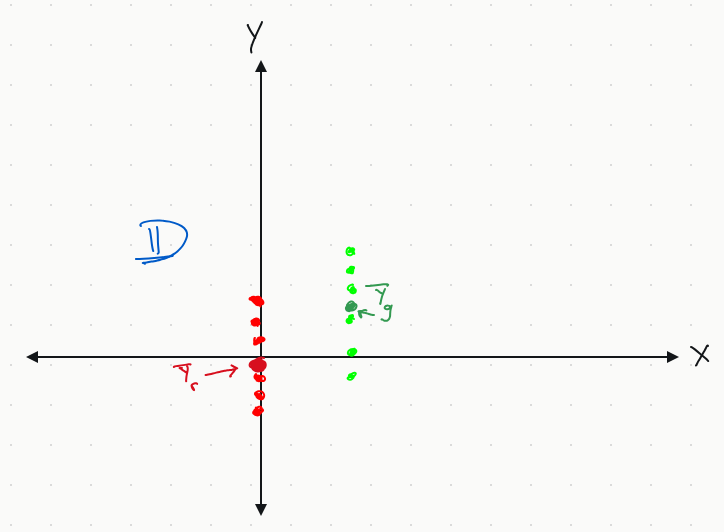
\includegraphics[width=0.6\textwidth]{anova-dataset}
		\caption{A data set $\mathbb{D}$ with $\mathcal{X}=\{\text{red}, \text{green}\}$ and
		$\mathbb{Y}=\mathbb{R}$.}
		\label{fig:anova-dataset}
	\end{figure}
	Take, for example, the data set $\mathbb{D}$ in Figure~\ref{fig:anova-dataset}. The inputs
	are ``red" and ``green", which is a categorical variable that we can encode as $0$
	and $1$, respectively. For these inputs, we have several points each with a different
	real-valued response. Figure~\ref{fig:anova-dataset} also highlights the values $\bar{y}_{\text{r}}$
	and $\bar{y}_{\text{g}}$ (that's $g$ for green, not the $g$ function), the average of the responses
	when limiting ourselves to the red and green inputs, respectively. A reasonable, yet naive model
	$g$ would predict that
	\begin{align}
		g(\text{red})&=\bar{y}_{\text{r}}\label{eqn:anova-g-1},\\
		g(\text{green})&=\bar{y}_{\text{g}}\label{eqn:anova-g-2}.
	\end{align}
	We will show that these are in fact the least squares estimates.
	This model is historically important, and it is called \textbf{ANOVA (ANalaysis Of VAriance)}.
	It is a linear ``regression" model for categorical variables. We proceed to
	prove our assertion about Equations~\ref{eqn:anova-g-1}~and~\ref{eqn:anova-g-2}.
	
	First, we will also introduce some notation. Let $n_r$ denote the number of red
	inputs and $n_g$ denote the number of green inputs. Also, let $p_r$ denote the proportion
	of red inputs and let $p_g$ denote the proportion of green inputs. Then
	we have the following relations:
	\begin{align*}
		n = n_r + n_g,\quad
		p_r = \frac{n_r}{n},\quad
		p_g = \frac{n_g}{n},\quad
		p_r=(1-p_g)
	\end{align*}
	Since we are encoding ``red" as $0$ and ``green" as $1$, we can use this notation to write
	\begin{align*}
		\bar{y}_r &= \frac{1}{n_r}\sum_{\{\,i \mid \ x_i=0\,\}}y_i\\
		\bar{y}_g &= \frac{1}{n_g}\sum_{\{\,i \mid \ x_i=1\,\} }y_i
	\end{align*}
	Next, we note that since $x_i\in\{0, 1\}$, it follows that $x_i=x_i^2$, so
	we have the following identities:
	\begin{align*}
		\bar{x} &= \frac{1}{n}\sum_{i=1}^{n}x_i=\frac{1}{n}\sum_{i=1}^{n}x_i^2\\
		\bar{x} &= \frac{1}{n}\sum_{i=1}^{n}x_i =\frac{1}{n}\sum_{\{\,i\mid\ x_i = 1\,\}}x_i=
		\frac{n_g}{n}=p_g\quad \iff \quad n\bar{x}=np_g
	\end{align*}
	We now invoke the equivalent of Equation~\ref{eqn:ols_b1_r} that we derived last time:
	\begin{align*}
		b_1 &= \frac{\sum_{i=1}^{n} x_iy_i - n\bar{x}\bar{y}}{\sum_{i=1}^{n}x_i^2-n\bar{x}^2}\\
		&=\frac{\underset{\{\,i \mid\ x_i = 1\,\}}{\sum} x_iy_i - n\bar{x}\bar{y}}{\sum_{i=1}^{n}x_i-n\bar{x}^2}
		\tag{Zeros do not contribute to sum, and $x_i=x_i^2$}\\
		&=\frac{n_g\cdot \frac{1}{n_g}\underset{\{\,i \mid\ x_i = 1\,\}}{\sum} y_i - np_g\bar{y}}{np_g - np_g^2}
		\tag{$x_i=1\implies x_i\cdot y_i=y_i$}\\
		&=\frac{np_g\bar{y}_g - np_g\bar{y}}{np_g - np_g^2}
		\tag{$n_g=np_g$}\\
		&=\frac{\bar{y}_g - \bar{y}}{1-p_g}\\
		&=\frac{\bar{y}_g - [p_g\bar{y}_g + (1-p_g)\bar{y}_r]}{1-p_g}\\
		&=\bar{y}_g-\bar{y}_r
	\end{align*}
	Now using Equation~\ref{eqn:ols_b0}:
	\begin{align*}
		b_0 &= \bar{y} - b_1\bar{x}\\
		&=(p_g\bar{y}_g+(1-p_g)\bar{y}_r)-(\bar{y}_g-\bar{y}_r)p_g\\
		&=p_g\bar{y}_g - p_g\bar{y}_g + \bar{y}_r - p_g\bar{y}_r + \bar{y}_rp_g\\
		&=\bar{y}_r
	\end{align*}
	In summary, the least squares estimate are given by
	\begin{align}
		b_0 &= \bar{y}_r\label{eqn:anova_b0}\\
		b_1 &=\bar{y}_g-\bar{y}_r\label{eqn:anova_b1}
	\end{align}
	Therefore, the linear least squares model is $g(x)=b_0+b_1x$. Now we can
	prove our assertion from Equations~\ref{eqn:anova-g-1}~and~\ref{eqn:anova-g-2}:
	\begin{align*}
		g(0) &= b_0 + b_1(0) = b_0 = \bar{y}_r,\\
		g(1) &= b_0 + b_1(1) = \bar{y}_r + (\bar{y}_g-\bar{y}_r) = \bar{y}_g,
	\end{align*}
	as we set out to show. This line is shown in Figure~\ref{fig:anova-least-squares}.
	Note that the intercept corresponds to the ``red" inputs, causing ``red" to take
	on the role of the reference variable. In particular, $b_0$ is $\bar{y}_r$, and
	$b_1$ is not $\bar{y}_g$, but rather, an offset from $\bar{y}_r$. This follows
	because we derived least squares by prepending to our design matrix $X$ a column
	of $1$'s, which we have been denoting as $\vec{\mathbf{1}}_n$. If, however, we
	omitted $\vec{\mathbf{1}}_n$ and instead used one binary column for each category
	(level), then each coefficient $b_0,b_1$ would correspond to the mean response for
	that level.
	\begin{figure}
		\centering
		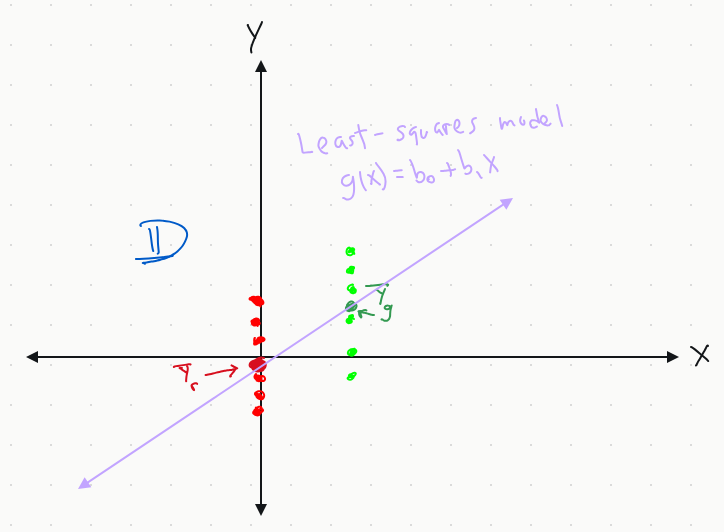
\includegraphics[width=0.5\textwidth]{anova-least-squares}
		\caption{A linear least squares fit for the data set in Figure~\ref{fig:anova-dataset}.}
		\label{fig:anova-least-squares}
	\end{figure}
	\section*{Multivariate Linear Least Squares Regression}
	We will now work towards extending the least square models to the multivariate
	case where $p>1$. Our set of candidate functions is the set of hyperplanes:
	\begin{align*}
		\mathcal{H} = \{\mathbf{x}\cdot \mathbf{w}=0:\ \mathbf{w}\in \mathbb{R}^{p+1}\}
	\end{align*}
	As a reminder, though we have $p$ features, we extend each input to length
	$p+1$ by prepending a $1$ entry to each input vector. This is simply
	for convenience, so that instead of writing $\mathbf{x}\cdot \mathbf{w}+b_0$,
	we can let $w_0=b_0$, $x_0=1$, and write $\mathbf{x}\cdot \mathbf{w}=0$.
	Thus, our matrix $X$ of inputs from $\mathbb{D}$ is of dimension $n\times (p+1)$,
	and looks like
	\begin{align*}
		X = \begin{bmatrix}
			1 & x_{1, 1} & x_{1, 2} & \cdots & x_{1, p}\\
			\vdots & \vdots & \vdots  &\cdots & \vdots\\
			1 & x_{n, 1} & x_{n, 2} & \cdots &  x_{n, p}
		\end{bmatrix}
	\end{align*}
	As in the case for $p=1$, the least squares algorithm seeks to find the
	vector $\mathbf{b}$ defining a hyperplane that minimizes the $SSE$ (the sum of
	squared errors):
	\begin{align*}
	\mathcal{A}(\mathbb{D}, \mathcal{H}) = \mathbf{b} =
	\underset{\mathbf{w}\in\mathbb{R}^{p+1}}{\text{argmin}}
	\{SSE\}
	\end{align*}
	where
	\begin{align*}
		SSE := \sum_{i=1}^{n}e_i^2
	\end{align*}
	We will use vector notation for our computations. Let
	\begin{align*}
		\mathbf{e} = \begin{bmatrix}
			e_1 \\
			e_2\\
			\vdots\\
			e_n
		\end{bmatrix},\quad
		\mathbf{y} = \begin{bmatrix}
			y_1 \\
			y_2\\
			\vdots\\
			y_n
		\end{bmatrix},\quad
		\mathbf{\hat{y}} = \begin{bmatrix}
			\hat{y}_1 \\
			\hat{y}_2\\
			\vdots\\
			\hat{y}_n
		\end{bmatrix},\quad
		\mathbf{w} = \begin{bmatrix}
			w_0\\
			w_1 \\
			w_2\\
			\vdots\\
			w_p
		\end{bmatrix}
	\end{align*}
	Since $\mathbf{e}=\mathbf{y}-\mathbf{\hat{y}}$, we can recast the equation for $SSE$:
	\begin{align*}
		SSE &= \sum_{i=1}^{n}e_i^2\\
		&=\mathbf{e}\cdot\mathbf{e}\\
		&=\mathbf{e}^\top \mathbf{e}\\
		&=(\mathbf{y}-\mathbf{\hat{y}})^\top(\mathbf{y} - \mathbf{\hat{y}})\\
		&=(\mathbf{y}^\top-\mathbf{\hat{y}}^\top)(\mathbf{y} - \mathbf{\hat{y}})\\
		&=\mathbf{y}^\top\mathbf{y}-\mathbf{y}^\top\mathbf{\hat{y}}-\mathbf{\hat{y}}^\top\mathbf{y}
		+\mathbf{\hat{y}}^\top\mathbf{\hat{y}}\\
		&=\mathbf{y}^\top\mathbf{y}-\mathbf{y}^\top\mathbf{\hat{y}}
		-(\mathbf{y}^\top\mathbf{\hat{y}})^\top
		+\mathbf{\hat{y}}^\top\mathbf{\hat{y}}
	\end{align*}
	Note we made use of the fact that $(A+B)^\top = A^\top + B^\top$, and that
	$(AB)^\top = B^\top A^\top$. Moreover, in general $A\neq A^\top$, but
	since $\mathbf{y}^\top \mathbf{\hat{y}}$ is a scalar, it does equal
	$(\mathbf{y}^\top\mathbf{\hat{y}})^\top$. Another relation that we will
	make use of is the fact that the prediction is given by matrix multiplication:
	\begin{align*}
		\hat{\mathbf{y}} = X\mathbf{w}
	\end{align*}
	Be sure to convince yourself of this. Putting these facts together, we can write
	\begin{align*}
		SSE &= 
		\mathbf{y}^\top\mathbf{y}-\mathbf{y}^\top\mathbf{\hat{y}}
		-(\mathbf{y}^\top\mathbf{\hat{y}})^\top
		+\mathbf{\hat{y}}^\top\mathbf{\hat{y}}\\
		&= \mathbf{y}^\top\mathbf{y}-2\mathbf{y}^\top\mathbf{\hat{y}}
		+\mathbf{\hat{y}}^\top\mathbf{\hat{y}}\\
		&=\mathbf{y}^\top\mathbf{y} - 2\mathbf{y}^\top (X\mathbf{w})+(X\mathbf{w})^\top(X\mathbf{w})\\
		&=\mathbf{y}^\top\mathbf{y}-2\mathbf{y}^\top X\mathbf{w}+\mathbf{w}^\top X^\top X\mathbf{w}
	\end{align*}
	To minimize the $SSE$, we now take $p+1$ partial derivatives, one with respect
	to each of $w_0,w_1,w_2,\ldots,w_p$, and we set them all to zero:
	\begin{align*}
		\frac{\partial}{\partial \mathbf{w}}[SSE] = \begin{bmatrix}
			\frac{\partial}{\partial w_0}[SSE]\\
			\frac{\partial}{\partial w_1}[SSE]\\
			\frac{\partial}{\partial w_2}[SSE]\\
			\vdots\\
			\frac{\partial}{\partial w_p}[SSE]\\
		\end{bmatrix}
		=\begin{bmatrix}
			0\\
			0\\
			0\\
			\vdots\\
			0
		\end{bmatrix}
		=\mathbf{0}_{p+1}
	\end{align*}
	In the case when $p=1$, we laboriously solved a system of equations to obtain the estimates
	$b_0$ and $b_1$. For the general case where $p>1$, we will resort to useful
	results from differential calculus and linear algebra to solve this system in one swoop.
	Next, we digress to mention these key results.
	\subsection*{Digression on Differential Calculus and Linear Algebra}
	\begin{proposition}
		Let $\mathbf{x}\in\mathbb{R}^n$, and let $a\in\mathbb{R}$ be a constant with
		respect to all entries of $\mathbf{x}$. Then
		\begin{align*}
			\frac{\partial}{\partial\mathbf{x}}[a] := \begin{bmatrix}
				\frac{\partial}{\partial x_1}[a]\\
				\frac{\partial}{\partial x_2}[a]\\
				\vdots\\
				\frac{\partial}{\partial x_n}[a]
			\end{bmatrix}
			=\begin{bmatrix}
				0\\
				0\\
				\vdots\\
				0
			\end{bmatrix}
			=\mathbf{0}_{n}
		\end{align*}
	\end{proposition}
	\begin{proposition}
		Let $\mathbf{a}\in\mathbb{R}^n$, where all entries are constant with respect to
		all entries of $\mathbf{x}$. Then
		\begin{align*}
			\frac{\partial}{\partial\mathbf{x}}[\mathbf{a}\cdot \mathbf{x}]=
			\frac{\partial}{\partial \mathbf{x}}[\mathbf{a}^\top \mathbf{x}]=\mathbf{a}
		\end{align*}
	\end{proposition}
	Next time we will show other key facts that we will use.
%	\printbibliography
\end{document}